\documentclass{article}
\usepackage{graphicx}
\usepackage[utf8]{inputenc}
\usepackage[vmargin=3.25cm,hmargin=3.25cm]{geometry}
\usepackage{hyperref}

\title{Finding Breakpoints of Viral Genomes using recan}
\author{Abinu Ajithan Jyothini}
\date{August 6th 2020}
\begin{document}

\maketitle
\section{Introduction}
In many different group of viruses recombination of genetic material is an important evolutionary process that generates much of genetic diversity.The patterns of recombination evident within the genomes of viruses can reveal lots of detail about their evolution and biology.Recombination is responsible for the evolution of viruses in response to selective forces present in a host environment \cite{perez2015recombination}. A better understanding of recombination events taking place in the genomes of viruses are useful for gaining in-sites about the biology of the viruses.The patterns of sequence exchange between viruses in different species can reveal otherwise undetectable ecological links between some species and barriers between others.\cite{martin2015rdp4}. The breakpoints of genomes can reveal details about mechanistic and biochemical processes regarding the recombination process.\cite{martin2015rdp4}.This project makes use of the python package 'recan'\cite{babin2020recan}(recombination analyzer) for constructing genetic distance plots and exploring them.Also, we make use of bio-python\cite{chapman2000biopython} package for plotting fasta sequences.
\section{Methods:}
\subsection{recan Python Package:}
recan is a python package developed for the recombination analysis and it provides a mean for constructing genetic distance plots and exploring them interactively.recan is based on python packages like Biopython, Pandas, Matplotlib, and Plotly libraries.
\section{Results}
\begin{figure}
    \centering
    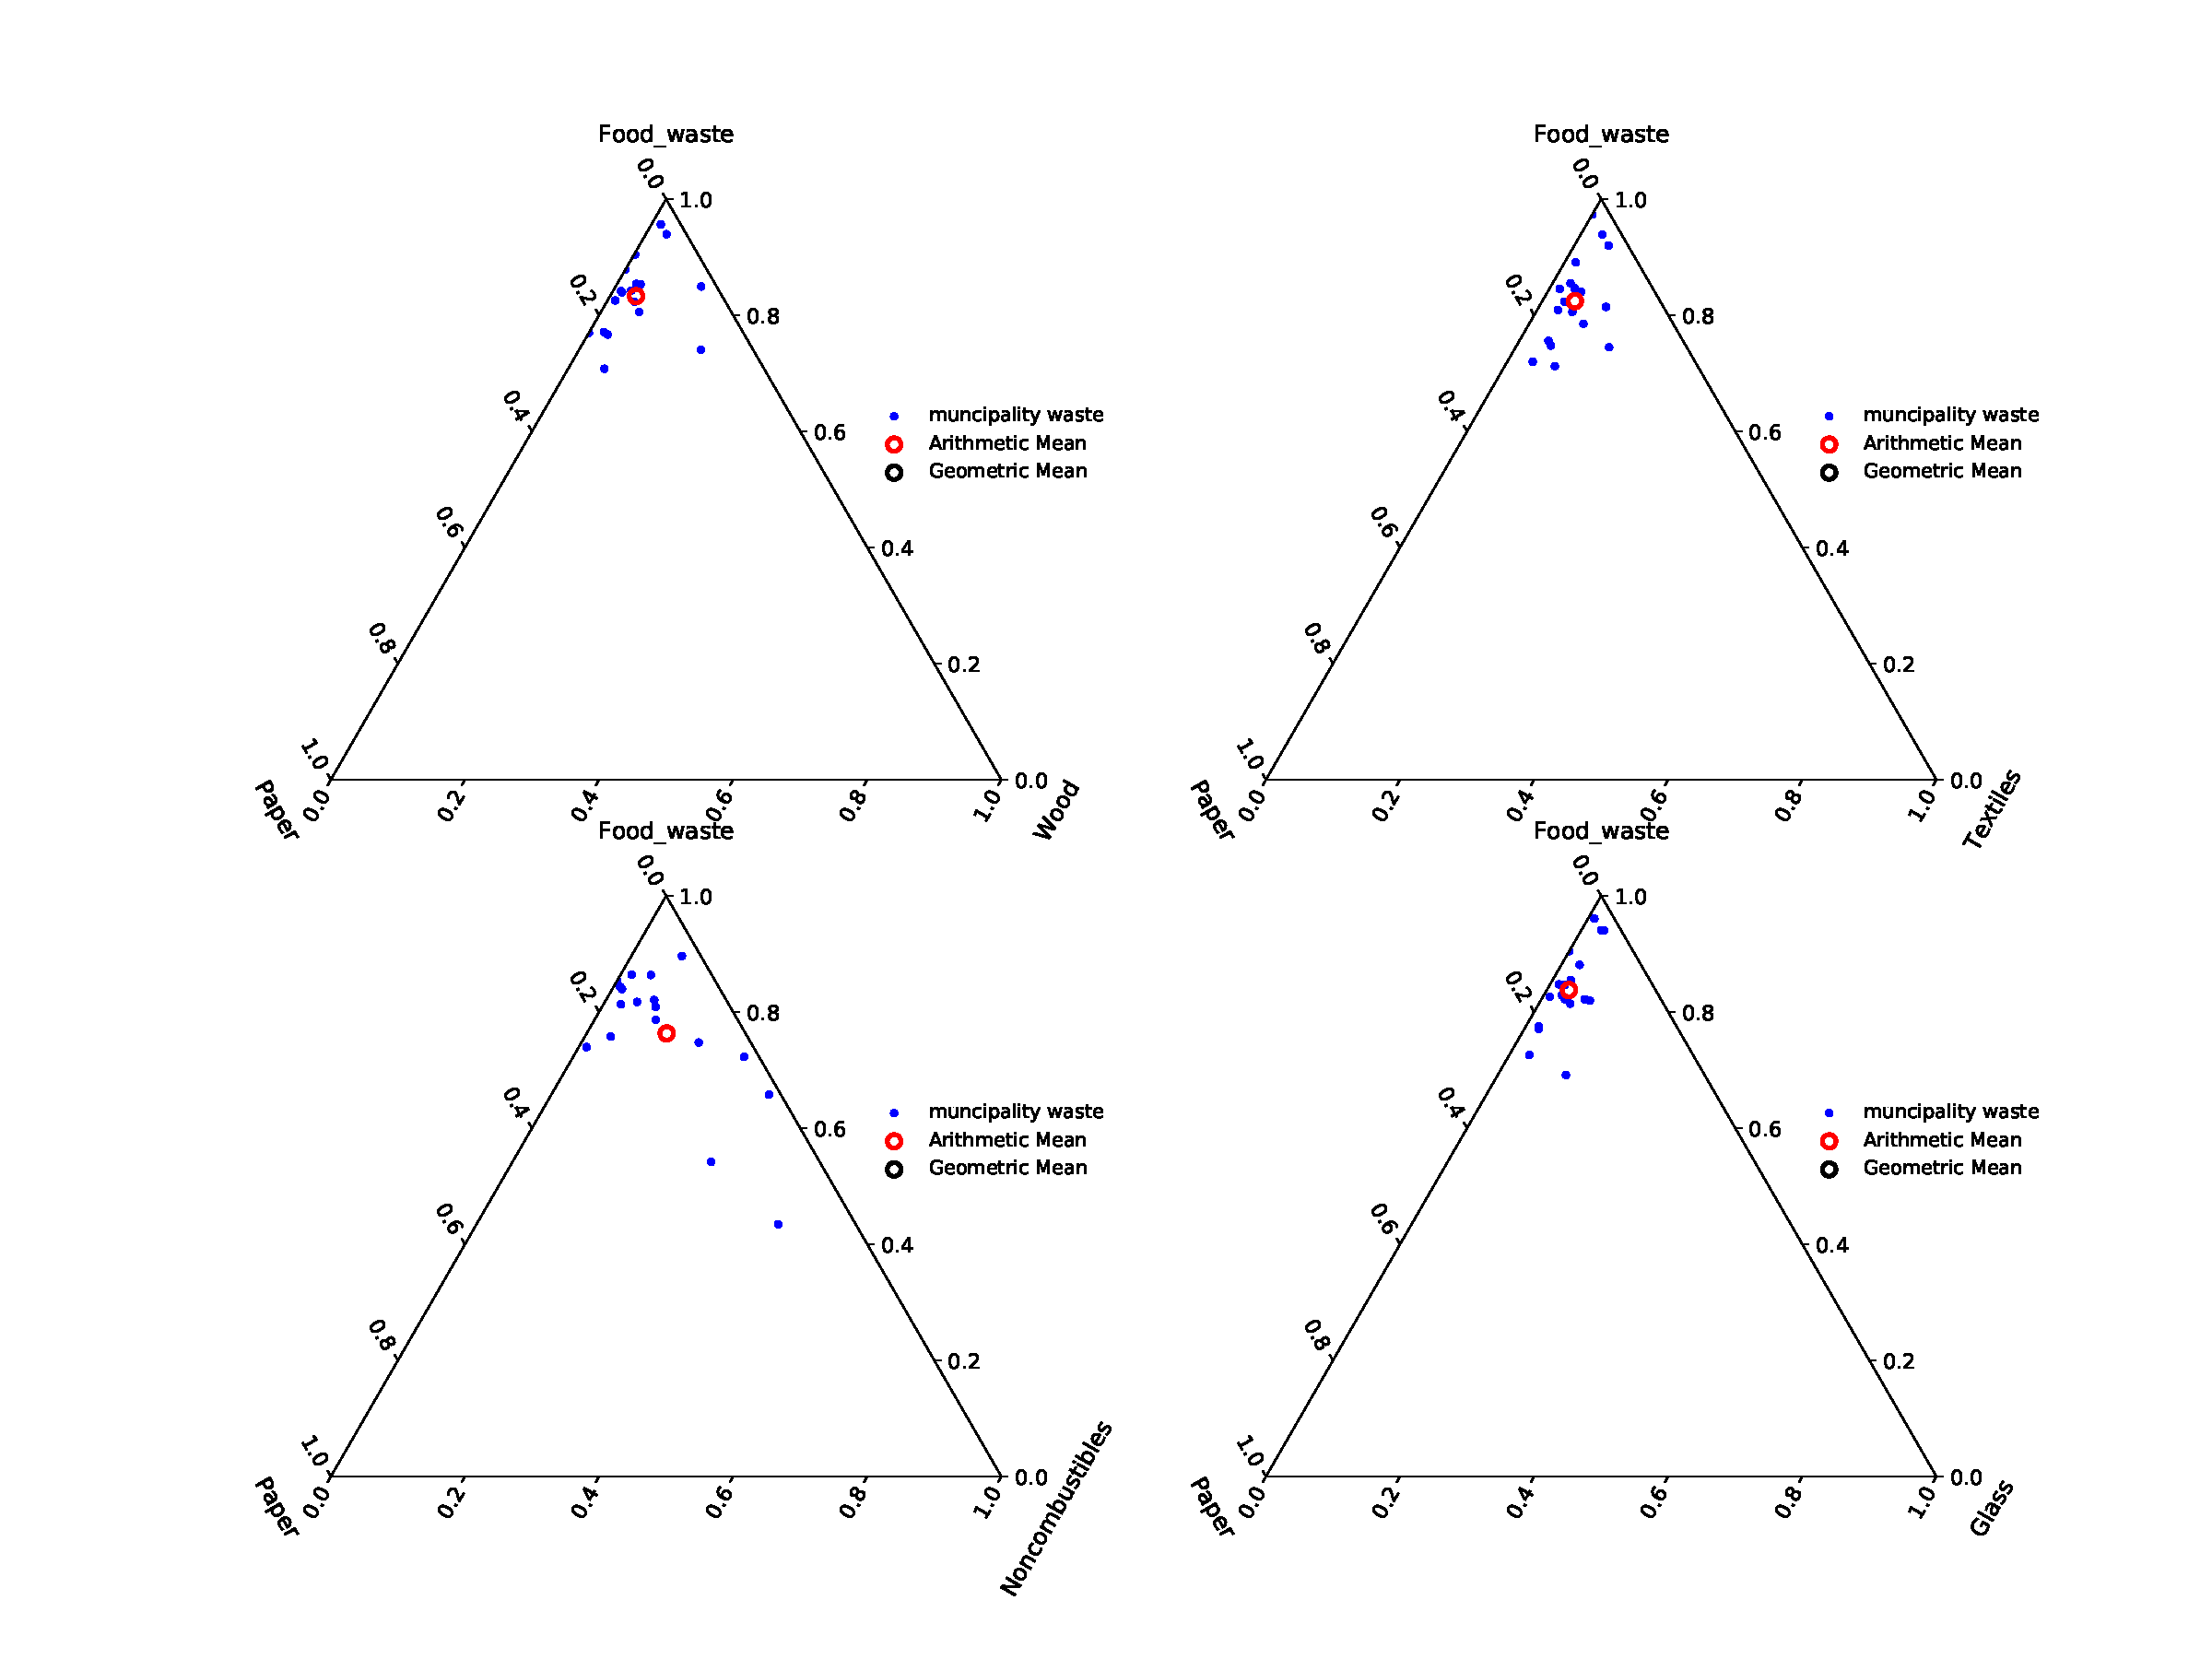
\includegraphics[width=0.9\textwidth]{ternary.png}
    \caption{Caption}
    \label{ternary}
\end{figure}

\begin{figure}
    \centering
    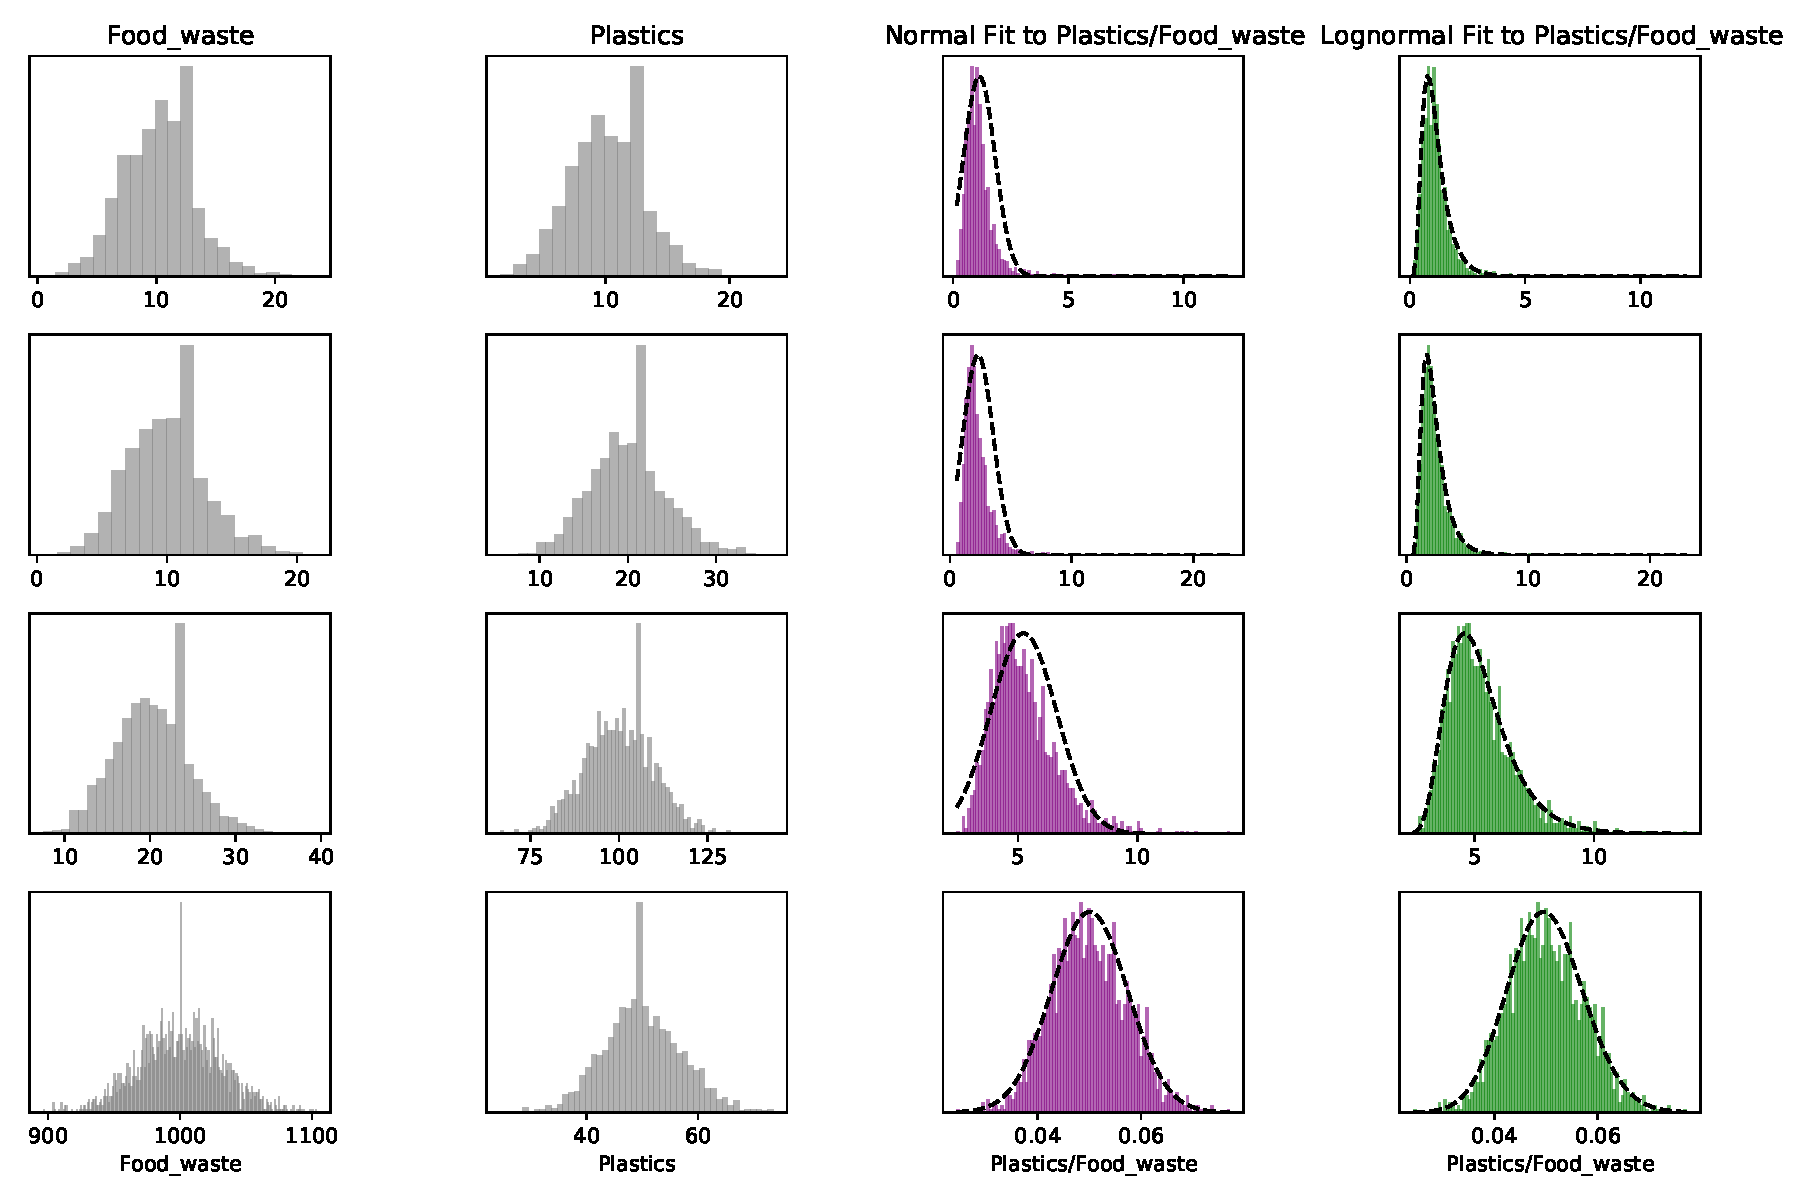
\includegraphics[width=0.9\textwidth]{lognormal.png}
    \caption{Caption}
    \label{ternary}
\end{figure}



\bibliography{rsc} 
\bibliographystyle{rsc}
\end{document}
